Im Folgenden Abschnitt soll die Analyse der aufgenommenen Daten erfolgen. 
Dafür wird zuerst darauf eingegangen, wie der störende Untergrund in den Messdaten, der durch die Spannungsversorgung der Xenonlampe hervorgerufen wird, beseitigt werden kann. 
Anschließend wird auf die Integration des Bunching Peaks eingegangen, indem zuerst über die Konstruktion einer Theoriefunktion und deren Fit und anschließend die Integration von dieser gesprochen wird. 
In diesem Zuge wird zudem kurz auf die Frage eingegangen, ob eine Integration der $g^{(2)}$-Funktion direkt oder eines Fits für die weitere Analyse sinnvoller ist. 
Danach wird erklärt, wie der Fehler auf die berechneten Integrale abgeschätzt wird. 
Nach diesen Schritten werden die ermittelten $\tau_c$ mit der theoretischen Erwartung aus \autoref{eq:tau_c_th} verglichen und diskutiert, ob ein Einfluss der Kabellänge auf $\tau_c$ vorliegt. 
Abschließend werden die erzielten Ergebnisse auf die Daten der H.E.S.S. Kampagne von 2022 angewandt. 

\subsection{Beiseitigung des niederfrequenten Störsignals in $g^{(2)}(\tau)$}
\label{ssec:Beseitigung des niederfrequenten Störsignals}
Wie in \autoref{ssec:mittelung und filter} angesprochen, ist das Signal welches den Bunching Peak beinhaltet überlagert von einem niederfrequenten Störsignal, welches von der Lampe hervorgerufen wird. 
Bevor das Integral des Peaks berechnet werden kann, muss dieses Störsignal entfernt werden. 
Betrachtet man Messreihen mit verschiedenen Kabellängen fällt auf, dass das Störsignal nicht exakt identisch ist. 
Stattdessen ist dieses immer leicht unterschiedlich. 
Für die Entfernung muss also das Störsignal aus jeder Messreihe separat bestimmt und entfernt werden. 
Eine Möglichkeit hierfür wäre einen Fit einer periodischen Funktion, z. B. $f(\tau) = a\cdot\mathrm{sin}(b(\tau-c))+d$ durchzuführen. 
Dies ist allerdings mit einigen Nachteilen verbunden. 
Betrachtet man das Störsignal (Abgebildet z. B. in \autoref{fig:gemittelte G2 vs g2}) genauer, fällt auf, dass dieses nicht symmetrisch ist. 
Um es voll zu erfassen, müsste $f(x)$ also noch um weitere Parameter ergänzt werden, was den Fit verkompliziert. 
Zusätzlich ist die Wahl der Fitfunktion letztlich arbiträr, da beliebige Parameter hinzugefügt werden können und keine Erwartung an die theoretsiche Form des Störsignals vorliegt. \\
Aufgrund der Tatsache, dass der Bunching Peak und das Störsignal aber um Größenordnungen verschiedene zeitliche Ausdehnungen haben (ersterer grob 100\,ns, letzteres etwa 10000\,ns), bietet es sich an das Muster des Störsignals im Frequenzraum zu extrahieren. 
Dafür wird ein Tiefpassfilter zweiter Ordnung verwendet, dessen Grenzfrequenz so gewählt wird, dass lediglich die niederfrequenten Anteile des Signals estrahiert werden. 
Das ermittelte Muster kann anschließend von $g^{(2)}(\tau)$ abgezogen werden, was den Offset entfernt und dafür sorgt, dass außerhalb des Bunching Peaks etwa $g^{(2)}\approx 0$ gilt. 
Für die Wahl der richtigen Grenzfrequenz hilft eine Blick auf \autoref{fig:lf_offset für verschiedene Grenzfrequenz}, in der abgebildet ist, wie das ermittelte Muster für verschiedene Grenzfrequenzen aussieht. 
\begin{figure}[h]
    \centering
    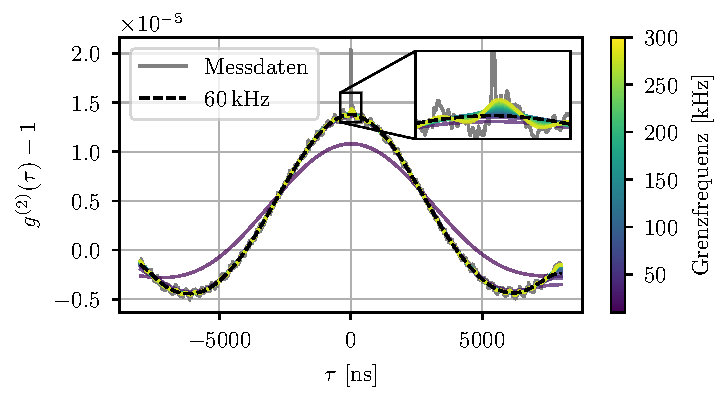
\includegraphics{images/Analysis/lf_offset.pdf}
    \caption{Gezeigt ist ein Vergleich der extrahierten Muster für verschiedene Grenzfrequenzen. In Grau ist die gemittelte $g^{(2)}$-Funktion, aufgenommen mit der Kabelkombination Airborne 5 $40\times 40$ Meter, dargestellt. Farbig hinterlegt sind die ermittelten Muster für verschiedene Grenzfrequenzen. Es ist offensichtlich, dass bei niedrigen Grenzfrequenzen Muster entstehen, die das Störsignal nicht voll erfassen (lila), und bei hohen Grenzfrequenzen (gelb) Muster entstehen, welche Amplitude vom Bunching Peak abschneiden. Eine gute Grenzfrequenz, die das Störsignal großflächig abdeckt und gleichzeitig keine feine Struktur erfasst liegt bei 60\,kHz und ist schwarz gestrichelt eingezeichnet.}
    \label{fig:lf_offset für verschiedene Grenzfrequenz}
\end{figure}
In der Abbildung ist ersichtlich, dass sowohl zu niedrige als auch zu hoch gewählte Grenzfrequenzen problemeatisch sind. 
Zu niedrig gewählte Greznfrequenzen sorgen dafür, dass das Störsignal nicht vollständig erfasst wird (vgl. lila Kurve in \autoref{fig:lf_offset für verschiedene Grenzfrequenz}). 
Je niedriger die Frequenz wird, desto mehr wird statt des gesamten Signals nur dessen Mittelwert extrahiert. 
Eine Subtraktion dieses Musters würde dann dazu führen, dass das Störsignal noch immer vorliegt und lediglich eine geringere Amplitude aufweist. 
Wählt man allerdings die Grenzfrequenz zu hoch, so werden Teile des höherfrequenten Signals der $g^{(2)}$-Funktion fälschlicherweise als Störsignal erkannt. 
Im Extremfall wird so ein Teil des Bunching Peaks bei der Subtraktion abgezogen, was das Ergebnis für $\tau_c$ verfälschen würde. 
Dies ist in \autoref{fig:lf_offset für verschiedene Grenzfrequenz} gelb eingezeichnet. \\
Es gilt also eine Grenzfrequenz zu finden, welche das Störsignal zwar großflächig vollständig erfasst, aber möglichst keinen Einfluss auf die Feinstruktur der Korrelationsfunktion hat. 
Diese Frequenz wird zu etwa 60\,kHz bestimmt. 
Zur Veranschaulichung ist das mit einer Grenzfrequenz von 60\,kHz ermittelte Muster schwarz gestrichelt in \autoref{fig:lf_offset für verschiedene Grenzfrequenz} eingezeichnet. \\

Nach dem Berechnen des Musters wird dieses von der $g^{(2)}$-Funktion abgezogen. 
Durch dieses Vorgehen, erhält man die Korrelationsfunktion, welche in \autoref{fig:g2-offset} dargestellt ist.
\begin{figure}[h]
    \centering
    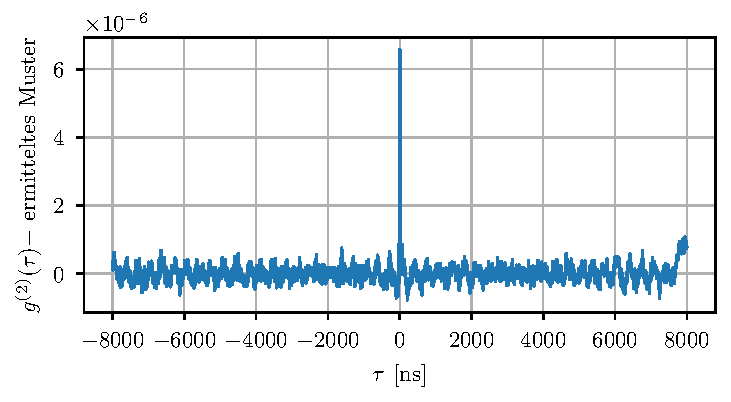
\includegraphics{images/Analysis/g2-lf_offset.pdf}
    \caption{Hier ist dargestellt, wie die $g^{(2)}$-Funktion nach Subtraktion des ermittleten niederfrequenten Störmusters aussieht. Der Bunching Peak sticht nun sehr klar aus dem Hintergrund heraus, welcher um den Wert 0 schwankt.}
    \label{fig:g2-offset}
\end{figure}
Es ist ersichtlich, dass die beschriebene Methode den niederfrequenten Offset im Signal gut entfernt. 
Ein weiterer Vorteil dieser Methode ist, dass der Hintergrund nun um den Wert 0 schwankt, sodass ein Offset in y-Richtung für die spätere Integration (und den Fit) nicht berücksichtigt werden muss. \\
Allerdings soll hier auch auf die Limitaitonen des erwähnten Vorgehens hingewiesen werden. 
Erstens ist auffällig, dass $g^{(2)}(\tau)$ für $|\tau|\gtrsim 6000\,\mathrm{ns}$ von der Schwankung um 0 abweicht und stattdessen wieder größer wird. 
Dies liegt daran, dass der Tiefpass diese Randregionen nicht mehr gut erfassen kann. 
Konkret ist auch schon in \autoref{fig:lf_offset für verschiedene Grenzfrequenz} ersichtlich, dass das extrahierte Muster in den Randregionen stets zu niedrig ist und daher nach der Subtraktion zu hohe Werte liefert. 
\todo{WArum? Fehlendes Signal rechts? finde quelle!}
Da der Bunching Peak aber für alle verwendeten Kabelkombinationen bei $\tau\approx 0$ liegt, ist die Auswirkung dieser Randbereiche auf $\tau_c$ vernachlässigbar. 
Trotzdem wird für alle folgenden Analyseabschnitte der Definitionsberiech der Offset-korrigierten $g^{(2)}$-Funktion auf $\tau\in[-6000,6000]\,\mathrm{ns}$ eingeschränkt, um einen Einfluss dieser Randeffekte (besonders auf den Fehler auf $\tau_c$, vgl. \todo{ref wenn fertig}) vermeiden zu können. 
Von größerem Belang ist allerdings die Wahl der Grenzfrequenz selbst. 
Wie oben beschrieben erfolgte diese hier anhand von visuellen Überlegungen anhand der $g^{(2)}$-Funktion und dem ermittelten Muster. 
Da sich aber für verschiedene Grenzfrequenzen leicht andere Werte des Musters bei $\tau\approx 0$ ergeben, wirken sich diese auch auf das Integral aus. 
Durch das Festlegen der Grenzfrequenz per Auge ergibt sich ein relativ großer Wertebereich an möglichen Grenzfrequenzen welche alle ähnlich plausibel erscheinen. 
Die hier gewählten 60\,kHz stellen so etwa die Mitte eines $\pm20\,\mathrm{kHz}$ breiten Bereichs dar. 
Der geschätzte systematische Fehler auf das Integral anhand der später entwickelten Integrationsstrategie liegt im niedrigen einstelligen Bereich. \\

Da dies, wie später klar wird, in der Größenordnung des statistischen Fehlers auf $\tau_c$ liegt, soll an dieser Stelle bereits auf die Notwendigkeit verwiesen werden, für weitere Labormessungen eine tiefergehende Untersuchung bezüglich der Wahl der Grenzfrequenz anzustellen. 
Diese sollte zum Ziel haben, eine besser gerechtfertigte Wahl für die Grenzfrequenz treffen zu können, und den systematischen Fehler, der durch die Festlegung dieser Frequenz entsteht besser zu quantifizieren. 
Da diese Untersuchungen allerdings den Rahmen dieser Arbeit überschreiten würden, wird im Folgenden von einer festen Grenzfrequenz von 60\,kHz ausgegangen, welche, wie in \autoref{fig:g2-offset} zu sehen, bereits zu guten Ergebnissen führt. 

\subsection{Fitfunktion}
\label{ssec:Fitfunktion}    
Nachdem der Offset der Korrelationsfunktion nun abgezogen ist, kann an das Integrieren dieser gedacht werden. 
Dafür sollen in einem späteren Abschitt verschiedene Integrationsmethoden und Integrationsbereiche miteinander verglichen werden, darunter auch die Integration eines Fits. 
Für diesen späteren Abschnitt ist es also nötig, eine Funktion zu finden, welche den Bunching Peak gut beschreibt. 
Dies soll das Ziel vom jetzigen Abschnitt sein. 

\subsubsection{Bisherige Herangehensweise}
\label{sssec:Fitfunktion - Bisherige Herangehensweise}
In der Arbeitsgruppe existieren bereits verschiedene Ideen darüber, welche Fitfunktion geeignet ist. 
So wurden für die ersten Labormessungen z. B. gemessene gemittelte Photonenpulse während der Ratenkalibration (vgl. \autoref{ssec:Datenaufnahme und Waveforms}) korreliert, linear interpoliert und an die Daten gefittet \cite{zmijaOpticalIntensityInterferometry2021}. 
Dies ergibt durchaus Sinn, da sich die Ausgangspulse der PMTs (wie in \autoref{ssec:Datenaufnahme und Waveforms} beschrieben) über einige Bins erstrecken und so das zeitlich sehr schmale Bunching Signal verwaschen. 
Die Erwartung an den Bunching Peak in den korrelierten Daten ist daher, dass er sich wie die PMT-Pulse über einige Bins erstreckt und etwa der Form der korrelierten mittleren Pulsform entspricht. \\
Eine weitere Herangehensweise liegt im Fit einer Gaußfunktion an das Signal. 
Dies entspricht der momentanen Herangehensweise der Arbeitsgruppe und wurde z. B. für die Auswertung der Daten der H.E.S.S. Kampagne von 2022 verwendet \cite{zmijaFirstIntensityInterferometry2023}. 
Vorteil dieser Methode ist die relativ einfache, analytische Funktion, welche an die Daten gefittet wird. 
Während bei der vorherigen Methode Daten korreliert und dann interpoliert wurden, um die Interpolationsfunktion daraufhin numerisch zu integrieren, kann bei einer Gaußfunktion auf eine simple Formel zurückgegriffen werden, sodass gilt:
\todo{cite}
\begin{equation}
    \tau_c^{\mathrm{meas}} = \sqrt{2\pi} a\sigma
\end{equation}
Hierbei sind $a$ die Amplitude und $\sigma$ die Breite der gefitteten Gaußfunktion. 
Dieses Vorgehen vereinfacht den Fit und erlaubt es, relativ einfach Fitparameter wie den Mittlelwert und die Breite $\sigma$ festzuhalten, was aufgrund niedriger Statistik z. B. für die Daten von 2022 nötig war \cite{zmijaFirstIntensityInterferometry2023}. 
Allerdings hat diese Methode auch einen Nachteil, welcher in \autoref{fig:g2-fit Gauß} visualisiert ist. 
Durch die Verwendung verschiedener Kabellängen und damit unterschiedlicher Dispersion des Signals für jeden Kanal, folgt für den Bunching Peak als Korrelation der beiden Kanäle, dass dieser asymetrisch ist. 
Diese Asymmetrie kann vom Gaußfit allerdings nicht vollständig erfasst werden -- es wird lediglich die mittlere Abweichung des Fits zu den Datenpunkten minimiert. 
\begin{figure}[h]
    \centering
    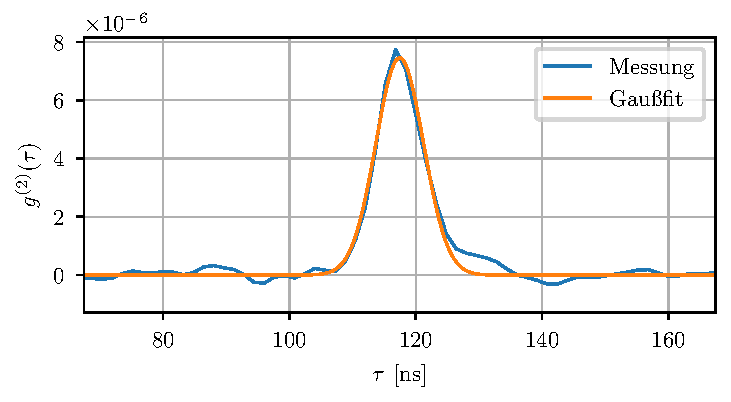
\includegraphics{images/Analysis/g2_gaussfit.pdf}
    \caption{Gezeigt sind die $g^{(2)}$-Funktion für die Messung mit 10\,m und 40\,m Kabeln des Typs Airborne 5. Zusätzlich ist der Fit einer Gaußfunktion eingezeichnet.}
    \label{fig:g2-fit Gauß}
\end{figure}
Wie in \autoref{fig:g2-fit Gauß} ersichtlich, werden besonders die Randbereiche des Peaks nciht vom Gaußfit erfasst. 
Aus der vorherigen Diskussion korrelierter benachbarter Bins und der Verbreiterung des Bunching Signals durch die Breite der PMT Pulse ist aber bereits ersichtlich geworden, dass auch diese Randbereiche Teil des Bunching Peaks sind. 
In der vorliegenden Arbeit soll daher, auch aufgrund der durch die Labormessungen höheren Statistik, von ersterer Methode ausgegangen werden. 
Die Schritte bis zur fertigen Fitfuntkion werden im Folgenden erläutert.

\subsubsection{Meine Herangehensweise}
\label{sssec:Fitfunktion - Meine Herangehensweise}
Wie bereits angesprochen, sehen die Pulse nach durchqueren unterschiedlich langer Kabel auch unterschiedlich aus. 
In \autoref{fig:mittlere Pulsform} sind zur Veranschaulichung zwei mittlere PMT-Pulse nach Durchlauf eines 40 bzw. 10\,m langen Airborne 5 Kabels dargestellt. 
Diese werden, wie in \autoref{ssec:Datenaufnahme und Waveforms} angesprochen, von der Aufnahmesoftware automatisch gespeichert. 
\begin{figure}[h]
    \centering
    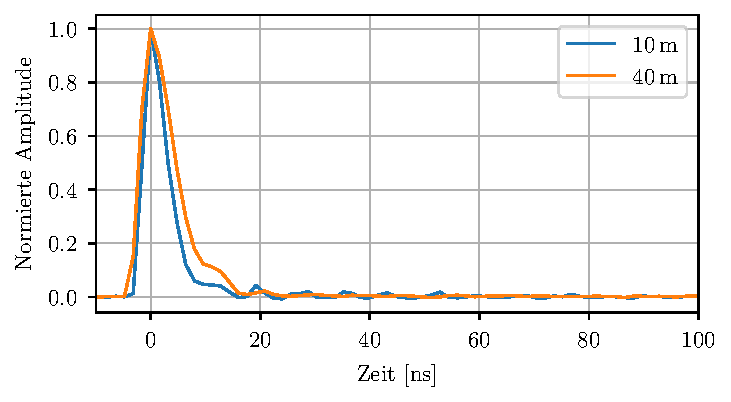
\includegraphics{images/Analysis/mean_pulseshapes.pdf}
    \caption{Gezeigt sind Asuschnitte der mittleren Pulsform bei Verwendung eines 40\,m bzw. 10\,m Airborne 5 Kabels. Es ist deutlich sichtbar, dass der orangene Puls deutlich breiter als der blaue ist, was an der erhöhten Dispersion im längeren Kabel liegt. Weiterhin wird eine stärkere Dämpfung, d. h. eine Abnahme der Amplitude für längere Kabel erwartet, was hier aber aufgrund der Normierung nicht direkt sichtbar ist.}
    \label{fig:mittlere Pulsform}
\end{figure}
Wie erwartet, ist der Puls durch das längere Kabel sichtbar verbreitert. 
Es lässt sich also bereits erahnen, dass die korrleation der beiden Pulse eine asymmetrische Form hat, welche zudem das Ringing der PMTs beeinhaltet, und somit dem Bunching Peak ähnlicher ist, als eine Gaußfunktion. 
\todo{was ist ringing}
Im Anschluss werden die beiden mittleren Pulse mit der selben Methode wie die Daten selbst, miteienander korreliert. 
Dieses Verfahren wurde bereits in \autoref{eq:korrelation} dargestellt. 
Der so erhaltene Vektor an Datenpunkten wird normiert, indem durch sein Maximum geteilt wird und so in der Zeit verschoben, das das Maximum bei $\tau=0$ liegt. 
Diese Schritte verändern die Korrelation nicht, vereinfachen aber später die Interpretation der Fitparameter. 
Da bisher noch keine Funktion, sondern lediglich Datenpunkte vorliegen, wird anschließend eine lineare Interpolation durchgeführt, um die Funktion $y(\tau)$ zu erhalten. 
Diese ist, zusammen mit dem Datenpunkten der korrelierten Pulsform in \autoref{fig:Interpolation} gezeigt. 
\begin{figure}[h]
    \centering
    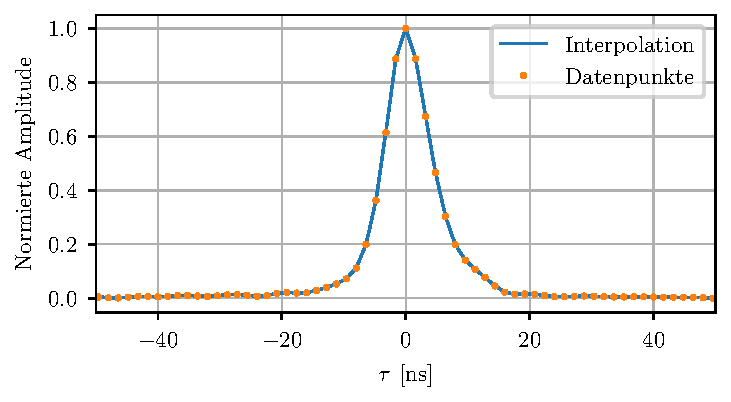
\includegraphics{images/Analysis/interpolation.pdf}
    \caption{Dargestellt ist das Ergebnis der diskreten Korrelation (orange) und die lineare Interpolation davon (blau).}
    \label{fig:Interpolation}
\end{figure}
Die so ermittelte Funktion $y(\tau)$ liese sich grundsätzlich unter Verwendung eines Offsets in x-Richtung $\tau_0$ und eines Amplitudenfaktors $a$ an den Bunching Peak fitten. 
Allerdings fällt auf, dass auf diese Weise der Fit deutlich zu schmal ist (etwa um den Faktor $1{,}4$). 
Dies liese sich grundsätztlich durch Einführung eines weiteren Fitparameters $b$, welcher die Funktion in x-Richtung streckt und staucht, beheben, mit welcher die Fitfukntion $f$ lauten würde: 
\begin{equation}
    f(\tau, a, b, \tau_0) = a\cdot y(b(\tau - \tau_0))
\end{equation}
Allerdings existiert ein physikalisch besser motivierter Weg. 
Die Verbreiterung des Bunching Peaks im Vergleich zu $y(\tau)$ ist auf eine zusätzliche statistische Schwankung des Bunching Peaks zurückzuführen. 
Aufgrund von Effekten wie der endlichen Samplerate der ADC und der zeitlichen Schwankung der PMT-Pulse ist jede korrleierte Datei leicht gegen eine andere verschoben. 
So wird nach Mittelung aller Dateien der resultierende Peak in der Zeit verwaschen und ist breiter als die Funktion $y(\tau)$, welche nur durch eine einzelne Messung entsteht. 
Die erwähnte zeitliche Schwankung ist unter dem Einfluss vieler unabhängiger statistischer Schwankungen durch den gesamten Messaufbau und kann daher aufgrund des zentralen Grenzwertsatzes als gaußverteilt angenommen worden. 
Um diesen Effekt in der Fitfuktion zu quantifizieren wird eine Vorgehensweise ähnlich der in \cite{lasseguesFieldIntensityCorrelations2022} gewählt, bei der die Funktion $y(\tau)$, welche der Theoriefuktion bei unendlicher Zeitauflösung entspricht, mit einer Gaußfunktion gefalten, welche über ihre Breite $\sigma$ Information über die Zeitauflösung enthält. 
Durch dieses Vorgehen lässt sich die Fitfunktion $f$ also wie folgt umschreiben:
\begin{equation}
    f(\tau, a, \sigma, \tau_0) = ay(\tau - \tau_0) * \mathrm{e}^{-\frac{\tau^2}{2\sigma^2}}
\end{equation}
Weil die verwendete Routine zur Faltung nur für Vektoren und nicht für Funktionen definiert ist, ergeben sich in der Auswertung noch leichte Abweichungen von dieser Vorgehensweise. 
So werden die linke und rechte Seite der Faltung erst in einem ausreichend großen und fein gewählten Intervall unter Einsetzung der Parameter $a=1$ und $\tau_0 = 0$ ausgewertet, woraufhin die diskrete Faltung der beiden Vektoren durchgeführt wird. 
Um anschließend wieder eine Funktion zu erhalten, welche für alle $\tau$ definiert ist, wird erneut eine lineare Interpolation durchgeführt und normiert, was zu Funktion $h$ führt. 
Schlussendlich ergibt sich die Fitfunktion also zu:
\begin{equation}
    f(\tau, a, \sigma, \tau_0) = ah(\tau- \tau_0, \sigma)
\end{equation} 
Durch die Variation der Parameter während der Fitroutine geht der Parameter $\sigma$ dann vor der Faltung ein, während die $a$ und $\tau_0$ der Einfachheit halber erst nach der Faltung und Interpolation eingehen. 
Durch die erwähnten Normierungs- und Verschiebungsschritte der Funktionen, welche die Funktion $f$ bilden, entspricht (bis auf für den Fit unwesentliche Abweichungen) $a$ nun der Amplitude des Fits und $\tau_0$ seinem Offset von $\tau=0$. 
Auf diese Weise sit eine Einschränkung der Fitparameter für die spätere Auswertung möglich, was die Konvergenz der Fits verbessert. 
$\sigma$ lässt sich als Zeitauflösung des gesamten Systems verstehen. 
Wie eine Variation des Fitparameters $\sigma$ die resultierende Funktion $f$ beeinflusst ist in \autoref{fig:Fitfuktion für verschiedene sigma} für $a=1$, $\tau_0=0$ dargestellt. 
\begin{figure}[h]
    \centering
    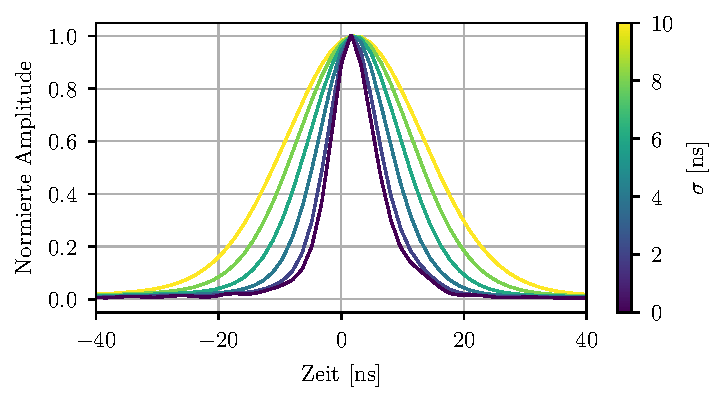
\includegraphics{images/Analysis/corr_pulses_diff_sigma.pdf}
    \caption{Dargestellt ist ein Ausschnitt der resultierenden Fitfunktion $f$ bei Variation des Fitparamters $\sigma$ ($a=1$, $\tau_0=0$). Für sehr niedrige $\sigma$ entspricht die Funktion praktisch der korrelierten Pulsform der PMTs und für größer werdende $\sigma$ nähert sich die Funktion immer mehr der Form einer Gaußfunktion an. Dies veranschaulicht die Interpretation von $\sigma$ als Zeitauflösung des Systems.}
    \label{fig:Fitfuktion für verschiedene sigma}
\end{figure}
Es ist ersichtlich, dass eine Erhöhung des Parameters $\sigma$ zu einer Verbreiterung der Fitfunktion führt, welche zudem immer glatter und gaußförmiger wird. 
Realsitische Werte für $\sigma$, welche sich in späteren Abschnitten ergeben werden, liegen im blauen Bereich der \autoref{fig:Fitfuktion für verschiedene sigma}. \\

Die Konstruktion und Verwendung der Fitfunktion wie oben beschrieben hat einige Vorteile. 
Wie bereits angesprochen, entspricht eine Faltung von einer Gaußfunktion, welche die Zeitauflösung enthält, mit der gemessenen erwarteten Peakform bei unendlicher Zeitauflösung am ehesten der theoretischen Erwartung an die Form des Bunching Peaks. 
Zudem wird durch dieses Vorgehen eine mögliche Asymmetrie und Ringing der PMTs berücksichtigt, was zu einer genaueren Bestimmung des Integrals und damit der Kohärenzzeit führen sollte. 
Durch die Veränderung der korrlierten Pulsform für jede Kabellängenkombination, ändert sich auch die Fitfunktion und bildet so die kabelabhängige Form des Bunching Peaks besser ab. 
Zusätzlich kann durch dieses Vorgehen die Zeitauflösung des Systems aus den gemessenen Daten bestimmt werden. 
Aus diesen Gründen wird im Folgenden, wann immer von der Fitfunktion die Rede ist, diese Funktion verwendet werden. 